% ===================================================================
% new_slides.tex: LCMFreq presentation — Metropolis style (cf. ref.tex)
% pdflatex + Vietnamese (T5 + babel), 16:9
% ===================================================================
\documentclass[9pt, aspectratio=169]{beamer}
\usetheme[progressbar=frametitle, block=fill]{metropolis}

% ---- Encoding & language ------------------------------------------
\usepackage[utf8]{inputenc}
\usepackage[T5]{fontenc}
\usepackage[vietnamese]{babel}
\usefonttheme{serif}

% ---- Packages ------------------------------------------------------
\usepackage{amsmath, amssymb}
\usepackage{booktabs}
\usepackage{array}
\usepackage{colortbl}
\usepackage{graphicx}
\usepackage{tikz}
\usetikzlibrary{arrows.meta, positioning, calc, fit, backgrounds, shapes.geometric}
\usepackage{listings}
\usepackage{appendixnumberbeamer}

% ---- Colours (cf. ref.tex) ------------------------------------------
\definecolor{deepblue}{HTML}{1B3A6B}
\definecolor{skyblue}{HTML}{3A7CA5}
\definecolor{accent}{HTML}{E76F51}
\definecolor{teal}{HTML}{2A9D8F}
\definecolor{violet}{HTML}{5E548E}
\definecolor{lightgray}{HTML}{F0F0F0}
\definecolor{optgreen}{HTML}{1B6B3A}

% ---- Metropolis tweaks ----------------------------------------------
\setbeamercolor{frametitle}{bg=deepblue}
\setbeamercolor{progress bar}{fg=accent,bg=skyblue!30}
\setbeamercolor{alerted text}{fg=accent}
\setbeamercolor{block title}{bg=skyblue!20,fg=deepblue}
\setbeamercolor{block body}{bg=lightgray}
\setbeamercolor{block title example}{bg=teal!20,fg=teal!80!black}
\setbeamercolor{block body example}{bg=teal!5}
\setbeamercolor{block title alerted}{bg=accent!20,fg=deepblue}
\setbeamercolor{block body alerted}{bg=accent!6}
\setbeamercolor{palette primary}{bg=deepblue}
\setbeamerfont{title}{size=\Large,series=\bfseries}
\setbeamerfont{subtitle}{size=\small}
\setbeamerfont{author}{size=\small}
\setbeamerfont{institute}{size=\footnotesize}
\setbeamerfont{date}{size=\footnotesize}
\setbeamerfont{frametitle}{size=\normalsize,series=\bfseries}
\metroset{sectionpage=progressbar}
\setbeamertemplate{title page}{%
  \vspace*{0.7cm}
  {\usebeamerfont{title}\usebeamercolor[fg]{title}\inserttitle\par}
  \vspace{0.35cm}
  {\usebeamerfont{subtitle}\usebeamercolor[fg]{subtitle}\insertsubtitle\par}
  \vspace{0.55cm}
  {\usebeamerfont{author}\insertauthor\par}
  \vspace{0.2cm}
  {\usebeamerfont{institute}\insertinstitute\par}
  \vspace{0.2cm}
  {\usebeamerfont{date}\insertdate\par}
}

% ---- Macros ----------------------------------------------------------
\newcommand{\hl}[1]{\textcolor{accent}{\textbf{#1}}}
\newcommand{\key}[1]{\textcolor{deepblue}{\textbf{#1}}}
\newcommand{\tc}[1]{\textcolor{teal}{#1}}
\newcommand{\opt}[1]{\textcolor{optgreen}{\textbf{#1}}}
\newcommand{\tikzmark}[1]{\tikz[remember picture,overlay,baseline]\coordinate (#1);}

% ---- Listings --------------------------------------------------------
\lstdefinelanguage{JuliaLite}{
  morekeywords={function,end,for,in,if,else,elseif,return,do,continue,let,begin},
  sensitive=true,
  morecomment=[l]\#,
  morestring=[b]"
}
\lstset{
  language=JuliaLite,
  basicstyle=\ttfamily\scriptsize,
  keywordstyle=\color{deepblue}\bfseries,
  commentstyle=\color{black!50},
  stringstyle=\color{teal},
  columns=fullflexible,
  escapeinside={(*@}{@*)},
  keepspaces=true,
  showstringspaces=false,
  frame=single,
  rulecolor=\color{deepblue!35},
  backgroundcolor=\color{lightgray},
  xleftmargin=0.5em,
  xrightmargin=0.5em,
  aboveskip=3pt,
  belowskip=3pt
}

% ---- TikZ styles -------------------------------------------------------
\tikzset{
  box/.style={rectangle,rounded corners=3pt,draw=#1,fill=#1!12,
    align=center,minimum height=0.85cm,font=\scriptsize\bfseries},
  boxt/.style 2 args={rectangle,rounded corners=3pt,draw=#1,fill=#2,
    align=center,minimum height=0.85cm,font=\scriptsize\bfseries},
  cell/.style={rectangle,draw=deepblue!70,fill=skyblue!12,minimum width=0.95cm,
    minimum height=0.8cm,font=\bfseries\small},
  bucket/.style={rectangle,rounded corners=2pt,draw=optgreen!70!black,fill=optgreen!8,
    minimum width=2.3cm,minimum height=0.8cm,align=center,font=\scriptsize},
  arrow/.style={-{Latex[length=1.8mm,width=1.2mm]},line width=0.65pt,#1},
  darrow/.style={-{Latex[length=1.8mm,width=1.2mm]},dashed,line width=0.65pt,#1},
  ptr/.style={-{Triangle[length=2.2mm,width=2mm]},line width=1.1pt,accent},
}

\title{LCMFreq}
\subtitle{Khai thác tập phổ biến bằng Backtracking, OccurrenceDeliver và Hypercube}
\author{Nhóm 01, CSC14004}
\institute{Trường Đại học Khoa học Tự nhiên, ĐHQG-HCM}
\date{HCMUS, học kỳ 2, năm học 2025--2026}

% ============================================================
\begin{document}
\maketitle

\begin{frame}{Nội dung trình bày}
  \setbeamertemplate{section in toc}[sections numbered]
  {\scriptsize\tableofcontents[hideallsubsections]}
\end{frame}

% ===================================================================
\section{Đặt vấn đề}
% ===================================================================

\begin{frame}{Bài toán Frequent Itemset Mining}
  \begin{columns}[T]
    \column{0.52\textwidth}
    Cho tập item $\mathcal I$ và database giao dịch
    $\mathcal D=\{T_1,\ldots,T_m\}$, $T_i\subseteq\mathcal I$.

    \vspace{0.3em}
    \textbf{Denotation}: $\mathcal T(P)=\{T_i\in\mathcal D : P\subseteq T_i\}$.\\
    \textbf{Frequency / support}: $\mathrm{sup}(P)=|\mathcal T(P)|$.\\
    $P$ là \hl{frequent} nếu $\mathrm{sup}(P)\geq\sigma$.

    \vspace{0.4em}
    \begin{block}{Hai tính chất nền tảng}
      \small
      $\mathcal T(P\cup Q)=\mathcal T(P)\cap\mathcal T(Q)$\\
      $P\subseteq Q \;\Rightarrow\; \mathcal T(Q)\subseteq\mathcal T(P)$
    \end{block}

    \column{0.44\textwidth}
    \centering
    \begin{tabular}{@{}cl@{}}
      \toprule
      TID & Items \\
      \midrule
      $T_1$ & $A,B,C,D$ \\
      $T_2$ & $A,B,D$ \\
      $T_3$ & $A,B,C$ \\
      $T_4$ & $B,C$ \\
      $T_5$ & $A,B,C,D$ \\
      \bottomrule
    \end{tabular}
    \vspace{0.3em}\\
    \footnotesize $\sigma=2$: $\mathrm{sup}(\{A,C\})=3\geq 2 \Rightarrow$ frequent.
  \end{columns}
\end{frame}

\begin{frame}{Tính đơn điệu $\Rightarrow$ cây sinh itemset không trùng}
  \begin{columns}[T]
    \column{0.40\textwidth}
    \small
    \textbf{Đơn điệu}: $P$ không frequent $\Rightarrow$ mọi superset của
    $P$ cũng không frequent.

    \vspace{0.3em}
    \textbf{tail$(P)$} = item chỉ số lớn nhất trong $P$. Backtracking chỉ
    thêm $e>\mathrm{tail}(P)$.

    \vspace{0.3em}
    \onslide<2->{\opt{Hệ quả}: mỗi itemset có \emph{đúng một} đường sinh
    duy nhất từ $\emptyset$ — không sinh trùng.}

    \column{0.58\textwidth}
    \centering
    \begin{tikzpicture}[scale=0.85,font=\scriptsize]
      \node[box=deepblue,minimum width=1.6cm] (root) at (0,0) {$\emptyset$};
      \node<2->[box=deepblue,minimum width=1.5cm] (A) at (-3.0,-1.3) {$A$};
      \node<2->[box=deepblue,minimum width=1.5cm] (C) at (0,-1.3) {$C$};
      \node<2->[box=deepblue,minimum width=1.5cm] (D) at (3.0,-1.3) {$D$};
      \node<3->[box=skyblue,minimum width=1.5cm] (AC) at (-3.8,-2.6) {$A,C$};
      \node<3->[box=skyblue,minimum width=1.5cm] (AD) at (-2.0,-2.6) {$A,D$};
      \node<3->[box=skyblue,minimum width=1.5cm] (CD) at (0.8,-2.6) {$C,D$};
      \node<4->[box=optgreen,minimum width=1.8cm] (ACD) at (-3.8,-3.9) {$A,C,D$};

      \draw<2->[arrow=deepblue] (root) -- node[left]{$A$} (A);
      \draw<2->[arrow=deepblue] (root) -- node[right]{$C$} (C);
      \draw<2->[arrow=deepblue] (root) -- node[right]{$D$} (D);
      \draw<3->[arrow=skyblue] (A) -- node[left]{$C$} (AC);
      \draw<3->[arrow=skyblue] (A) -- node[right]{$D$} (AD);
      \draw<3->[arrow=skyblue] (C) -- node[right]{$D$} (CD);
      \draw<4->[arrow=optgreen] (AC) -- node[left]{$D$} (ACD);
    \end{tikzpicture}
    \vspace{0.1em}\\
    \onslide<4->{\footnotesize\color{black!55} $\{A,C,D\}$ chỉ sinh được qua
    $A\to C\to D$, không qua $C\to A\to D$ hay $D\to A\to C$.}
  \end{columns}
\end{frame}

% ===================================================================
\section{Khung Backtracking}
% ===================================================================

\begin{frame}{Apriori vs.\ Backtracking}
  \centering
  \begin{tikzpicture}[font=\scriptsize, node distance=0.4cm]
    \node[box=skyblue,text width=4.6cm,minimum height=2.4cm] (ap) at (0,0)
      {\textbf{Apriori (level-by-level)}\\[2pt]
       sinh $\mathcal D_k$ từ toàn bộ $\mathcal D_{k-1}$\\[2pt]
       \hl{phải giữ cả $\mathcal D_{k-1}$} trong bộ nhớ\\[2pt]
       $+$ dễ đếm support theo lô};
    \node[box=optgreen,text width=4.6cm,minimum height=2.4cm,right=2.0cm of ap] (bt)
      {\textbf{Backtracking (DFS)}\\[2pt]
       sinh đệ quy từ nghiệm hiện tại $P$\\[2pt]
       \opt{chỉ giữ $P$ trên ngăn xếp} — tiết kiệm bộ nhớ\\[2pt]
       $-$ đếm support từng candidate riêng lẻ, tốn thời gian};
  \end{tikzpicture}

  \vspace{0.5em}
  \begin{quote}
  \small\textit{``Apriori algorithms use much memory for storing
  $\mathcal D_k$ \dots\ backtracking algorithms use less memory \dots\
  However, apriori algorithms have advantages for the frequency
  counting.''} — Uno, Kiyomi, Arimura (2004)
  \end{quote}
  \centering\small LCMFreq = khung \opt{Backtracking} $+$ hai kỹ thuật bù lại
  điểm yếu đếm support.
\end{frame}

\begin{frame}[fragile]{Khung thuật toán BackTracking}
  \begin{columns}[T,onlytextwidth]
    \begin{column}{0.46\textwidth}
\begin{lstlisting}
BackTracking(P):
    output P
    for e in I, e > tail(P):
        if P union {e} la frequent:
            BackTracking(P union {e})
\end{lstlisting}
    \end{column}
    \begin{column}{0.5\textwidth}
      \small Mỗi lượt gọi: xuất $P$, rồi thử mở rộng với từng $e>\mathrm{tail}(P)$.

      \vspace{0.4em}
      \onslide<2->{LCMFreq giữ nguyên khung này, chỉ thay hai bước bên trong:}
      \begin{itemize}
        \item<2-> \tc{OccurrenceDeliver} — đếm support nhanh hơn
        \item<3-> \tc{HypercubeDecomposition} — xuất theo lô
      \end{itemize}
    \end{column}
  \end{columns}
\end{frame}

\begin{frame}{Ba kỹ thuật của LCMFreq trên khung Backtracking}
  \centering
  \resizebox{0.92\linewidth}{!}{%
  \begin{tikzpicture}[font=\footnotesize, node distance=0.5cm]
    \node[box=deepblue,minimum width=2.2cm] (p) at (0,0) {$P$};
    \node<2->[boxt={teal}{teal!12},minimum width=2.6cm,right=1.4cm of p] (bucket)
      {Buckets\\$\mathrm{Bucket}[e]$};
    \node<3->[boxt={skyblue}{skyblue!12},minimum width=2.8cm,right=1.4cm of bucket] (h)
      {$H(P)$\\item miễn phí};
    \node<4->[boxt={optgreen}{optgreen!12},minimum width=2.8cm,right=1.4cm of h] (out)
      {Xuất $P\cup Q$\\$Q\subseteq S'$, một lượt};

    \draw<2->[arrow=teal] (p) -- node[above]{\scriptsize Occ.Deliver} (bucket);
    \draw<3->[arrow=skyblue] (bucket) -- node[above]{\scriptsize cùng support} (h);
    \draw<4->[arrow=optgreen] (h) -- node[above]{\scriptsize Hypercube} (out);
  \end{tikzpicture}}

  \vspace{0.05em}
  \begin{itemize}\setlength\itemsep{0.15em}
    \item \key{1. Backtracking}: prefix $P$, chỉ thêm $e>\mathrm{tail}(P)$.
    \item<2-> \tc{2. OccurrenceDeliver}: duyệt $\mathcal T(P)$ một lần, rải vào bucket
      của mọi candidate cùng lúc.
    \item<3-> \tc{3. Hypercube}: item không làm giảm denotation $\Rightarrow$ xuất
      cả tổ hợp một lượt, không đệ quy riêng.
  \end{itemize}
\end{frame}

% ===================================================================
\section{Đếm support hiệu quả}
% ===================================================================

\begin{frame}{Down project: giao hai danh sách TID bằng hai con trỏ}
  \begin{equation}
    \mathcal T(P_1\cup P_2)=\mathcal T(P_1)\cap\mathcal T(P_2)
    \quad\text{tính trong } O(|\mathcal T(P_1)|+|\mathcal T(P_2)|)
  \end{equation}
  \centering
  \begin{tikzpicture}[font=\small]
    % T1 row
    \node[font=\scriptsize\bfseries] at (-1.0,2.05) {$\mathcal T(P_1)$};
    \foreach \v/\x [count=\i] in {1/0,3/1,5/2,7/3,9/4} {
      \node[cell] (t1\i) at (\x*1.35,1.6) {\v};
    }
    % T2 row
    \node[font=\scriptsize\bfseries] at (-1.0,0.05) {$\mathcal T(P_2)$};
    \foreach \v/\x [count=\j] in {3/0,5/1,6/2,9/3,10/4} {
      \node[cell] (t2\j) at (\x*1.35,-0.4) {\v};
    }
    % output row placeholder
    \node[font=\scriptsize\bfseries] at (-1.0,-1.85) {Giao};
    \node<2->[bucket,minimum width=1.05cm] (o3) at (1.10,-1.85) {3};
    \node<3->[bucket,minimum width=1.05cm] (o5) at (2.75,-1.85) {5};
    \node<5->[bucket,minimum width=1.05cm] (o9) at (4.40,-1.85) {9};

    % pointers i,j: exact-slide so each step shows only current position
    \node<1>[ptr] at (0,0.82) {$\blacktriangle$}; \node<1>[ptr] at (0,-1.12) {$\blacktriangledown$};
    \node<2>[ptr] at (1.35,0.82) {$\blacktriangle$}; \node<2>[ptr] at (0,-1.12) {$\blacktriangledown$};
    \node<3>[ptr] at (2.7,0.82) {$\blacktriangle$}; \node<3>[ptr] at (1.35,-1.12) {$\blacktriangledown$};
    \node<4>[ptr] at (4.05,0.82) {$\blacktriangle$}; \node<4>[ptr] at (2.7,-1.12) {$\blacktriangledown$};
    \node<5>[ptr] at (4.05,0.82) {$\blacktriangle$}; \node<5>[ptr] at (4.05,-1.12) {$\blacktriangledown$};
    \node<6>[ptr] at (5.4,0.82) {$\blacktriangle$}; \node<6>[ptr] at (4.05,-1.12) {$\blacktriangledown$};
  \end{tikzpicture}

  \vspace{0.4em}
  \centering\small
  \only<1>{$i{=}1,j{=}1$: \;$1<3$ $\Rightarrow$ tăng $i$.}%
  \only<2>{$i{=}2,j{=}1$: \;$3=3$ $\Rightarrow$ \opt{xuất 3}, tăng cả hai.}%
  \only<3>{$i{=}3,j{=}2$: \;$5=5$ $\Rightarrow$ \opt{xuất 5}, tăng cả hai.}%
  \only<4>{$i{=}4,j{=}3$: \;$7>6$ $\Rightarrow$ tăng $j$.}%
  \only<5>{$i{=}4,j{=}4$: \;$7<9$ $\Rightarrow$ tăng $i$.}%
  \only<6>{$i{=}5,j{=}4$: \;$9=9$ $\Rightarrow$ \opt{xuất 9}, tăng cả hai. $i$ vượt
    cuối $\Rightarrow$ dừng.}\\
  \onslide<6->{\footnotesize\color{black!55} Mỗi phần tử của $T(P_1)$ và
    $T(P_2)$ chỉ bị con trỏ đi qua \textbf{đúng một lần} $\Rightarrow$
    $O(|T(P_1)|+|T(P_2)|)$ bước.}
\end{frame}

\begin{frame}{Vấn đề khi áp dụng down project cho Backtracking}
  Backtracking luôn thêm \emph{đúng một item} mỗi lượt $\Rightarrow$ cặp tách
  duy nhất khả dụng là $P_1=P$, $P_2=\{e\}$. Với $k$ candidate $e>\mathrm{tail}(P)$:
  \begin{equation}
    O\!\left(\sum_{e>\mathrm{tail}(P)} \bigl(|\mathcal T(P)|+|\mathcal T(\{e\})|\bigr)\right)
  \end{equation}
  \centering
  \begin{tikzpicture}[font=\scriptsize,scale=0.82,transform shape]
    \foreach \name/\x/\h/\col in {B/0/1.6/skyblue, C/1.6/1.4/teal, D/3.2/1.2/accent} {
      \draw[fill=\col!20,draw=\col] (\x,0) rectangle (\x+1.2,\h);
      \node at (\x+0.6,\h+0.25) {$|T(P)|{+}|T(\{\name\})|$};
    }
    \draw[fill=optgreen!15,draw=optgreen] (4.8,0) rectangle (6.0,4.5);
    \node[align=center] at (5.4,2.25) {\textbf{21 bước}\\(3 lần đọc lại\\$T(P)$)};
  \end{tikzpicture}\\
  \vspace{0.2em}
  \footnotesize\color{black!60} $|\mathcal T(P)|$ bị cộng lặp lại cho \emph{từng}
  candidate, dù không đổi giữa các lần đó — đây là phần lãng phí mà
  OccurrenceDeliver loại bỏ.
\end{frame}

\begin{frame}[fragile]{OccurrenceDeliver: duyệt $\mathcal T(P)$ đúng một lần}
  \begin{columns}[T,onlytextwidth]
    \begin{column}{0.42\textwidth}
\begin{lstlisting}
OccurrenceDeliver(D, P):
  for e > tail(P):
      Bucket[e] := empty
  for t in T(P):
      for e in t, e > tail(P):
          insert t into Bucket[e]
  # Bucket[e] = T(P union {e})
\end{lstlisting}
      \small
      \begin{equation}
        O\!\Bigl(|\mathcal T(P)|+\!\!\sum_{e>\mathrm{tail}(P)}\!\!|\mathcal T(P\cup\{e\})|\Bigr)
      \end{equation}
    \end{column}
    \begin{column}{0.55\textwidth}
      \centering
      \begin{tikzpicture}[font=\small,scale=0.92,transform shape]
        \node[font=\bfseries\scriptsize] at (1.5,5.7) {$\mathcal T(\{A\})=\{t_1,t_3,t_5\}$};
        \node<1->[cell,minimum width=2.6cm] (t1) at (1.5,4.9) {$t_1=\{A,B,C\}$};
        \node<2->[cell,minimum width=2.6cm] (t3) at (1.5,2.7) {$t_3=\{A,C,D\}$};
        \node<3->[cell,minimum width=2.6cm] (t5) at (1.5,0.5) {$t_5=\{A,B,D\}$};

        \node[bucket] (bB) at (6.8,4.9) {\textbf{Bucket[B]}\\$t_1,t_5$\\sup$=2$};
        \node[bucket] (bC) at (6.8,2.7) {\textbf{Bucket[C]}\\$t_1,t_3$\\sup$=2$};
        \node[bucket] (bD) at (6.8,0.5) {\textbf{Bucket[D]}\\$t_3,t_5$\\sup$=2$};

        \draw<1->[arrow=deepblue] (t1.east) -- node[above,pos=0.4]{$B$} (bB.west);
        \draw<1->[arrow=deepblue] (t1.east) to[out=0,in=160] node[above,pos=0.3]{$C$} (bC.west);
        \draw<2->[arrow=teal] (t3.east) to[out=0,in=200] node[below,pos=0.3]{$C$} (bC.west);
        \draw<2->[arrow=teal] (t3.east) to[out=0,in=160] node[above,pos=0.3]{$D$} (bD.west);
        \draw<3->[arrow=accent] (t5.east) to[out=0,in=200] node[below,pos=0.25]{$B$} (bB.west);
        \draw<3->[arrow=accent] (t5.east) -- node[below,pos=0.35]{$D$} (bD.west);
      \end{tikzpicture}
    \end{column}
  \end{columns}
  \onslide<4->{\centering\footnotesize\color{black!55}
  6 bước (so với 21 ở down project) — mỗi giao dịch chỉ "rải" đúng một lần,
  cho \emph{cả ba} candidate cùng lúc.}
\end{frame}

\begin{frame}{Bất biến sau khi deliver}
  \begin{block}{Bất biến cần nhớ}
    \begin{equation}
      \mathrm{Bucket}[e]=\{t\in\mathcal T(P): e\in t\}=\mathcal T(P\cup\{e\})
      \quad\Rightarrow\quad
      \mathrm{sup}(P\cup\{e\})=|\mathrm{Bucket}[e]|
    \end{equation}
  \end{block}
  \small Bucket \emph{là} denotation của $P\cup\{e\}$ — dùng được ngay cho:
  kiểm tra minsup, đệ quy tiếp, và (slide sau) phát hiện item miễn phí trong
  HypercubeDecomposition — không cần tính lại gì cả.

  \vspace{0.5em}
  \begin{exampleblock}{Vì sao không dùng bitmap (Uno et al., 2004)}
    \small\textit{``This method has a disadvantage for sparse datasets \dots\
    not good for sparse large datasets.''} LCMFreq gốc dùng mảng số nguyên.
    \opt{Bản tối ưu của nhóm} đổi sang \texttt{BitArray}: tăng tốc mạnh trên
    dataset dày đặc (Chess, Pumsb), khiêm tốn hơn trên dataset thưa (Retail)
    — đúng như nhận định trên.
  \end{exampleblock}
\end{frame}

% ===================================================================
\section{HypercubeDecomposition}
% ===================================================================

\begin{frame}[fragile]{$H(P)$: item miễn phí và xuất theo lô}
  \begin{block}{Định nghĩa (Uno et al., 2004, Mục 3.3)}
    \small $H(P)=\{e>\mathrm{tail}(P): \mathcal T(P)=\mathcal T(P\cup\{e\})\}$.
    Kiểm tra $e\in H(P)$ chỉ cần so độ dài: $|\mathrm{Bucket}[e]|=|\mathcal T(P)|$
    — \emph{đã có sẵn} sau OccurrenceDeliver.
  \end{block}

  \begin{columns}[T,onlytextwidth]
    \begin{column}{0.46\textwidth}
\begin{lstlisting}
H = filter(e ->
    length(Bucket[e]) == support_P,
    F)
S_prime = S union H
for Q subset of S_prime:
    output P union Q with support_P
\end{lstlisting}
    \end{column}
    \begin{column}{0.50\textwidth}
      \centering
      \begin{tikzpicture}[font=\scriptsize, node distance=0.5cm]
        \node[box=deepblue,minimum width=2.4cm] (p) {$P$, $S'=S\cup H(P)$};
        \node<2->[box=optgreen,minimum width=4.6cm,below=0.7cm of p]
          {Với mọi $Q\subseteq S'$: $P\cup Q$ frequent\\
           $\Rightarrow$ xuất $2^{|S'|}$ itemset trong \textbf{một} lượt};
      \end{tikzpicture}
    \end{column}
  \end{columns}

  \vspace{0.4em}
  \onslide<3->{\centering\small\textit{``This saves about $2^{|H(P)|}$ times
  of the frequency counting.''} — Uno et al. (2004). Đệ quy tiếp chỉ với
  $e\notin S'$; các item trong $S'$ bị loại để tránh sinh lại.}
\end{frame}

\begin{frame}{Vì sao xuất theo lô vẫn đúng và đủ}
  \begin{itemize}
    \item $e\in H(P)\Rightarrow\mathcal T(P\cup\{e\})=\mathcal T(P)$; áp dụng
      liên tiếp cho mọi $e\in Q\subseteq S'$ $\Rightarrow$
      $\mathcal T(P\cup Q)=\mathcal T(P)$.
    \item Đúng với \emph{mọi} $Q\subseteq S'$, kể cả $Q=\emptyset$ (chính là
      $P$) và $Q=S'$.
    \item Không cần đệ quy riêng vào $S'$: đệ quy vào đó chỉ cho lại đúng
      những itemset đã xuất.
  \end{itemize}
  \begin{alertblock}{Trực giác}
    Hypercube không bỏ sót, không thêm sai: chỉ \emph{gom} các node cùng
    denotation (cùng support) để xuất một lần, giảm số nhánh phải đi qua mà
    vẫn cho đúng tập frequent itemset như đệ quy đầy đủ.
  \end{alertblock}
\end{frame}

% ===================================================================
\section{Pseudo-code và ví dụ chạy tay}
% ===================================================================

\begin{frame}[fragile]{Pseudo-code LCMFreq đầy đủ}
  \begin{columns}[T,onlytextwidth]
    \begin{column}{0.62\textwidth}
\begin{lstlisting}
LCMFreqBase(P, tids_P, F, S):
(*@\tikzmark{lcmODstart}@*)    support_P = length(tids_P)
    Bucket[e] = [] for each e in F
    for tid in tids_P:                  # OccDeliver
        for item in transaction[tid]:
            if item in F:
                push tid into Bucket[item](*@\tikzmark{lcmODend}@*)

(*@\tikzmark{lcmHstart}@*)    H = {e in F : length(Bucket[e]) == support_P}
    S_prime = S union H                  # Hypercube(*@\tikzmark{lcmHend}@*)

(*@\tikzmark{lcmOUTstart}@*)    for Q subset of S_prime:
        output P union Q with support_P(*@\tikzmark{lcmOUTend}@*)

(*@\tikzmark{lcmRECstart}@*)    for e in F, e > tail(P), e not in S_prime:
        if length(Bucket[e]) >= minsup:
            LCMFreqBase(P+{e}, Bucket[e], F_next, S_prime)(*@\tikzmark{lcmRECend}@*)
\end{lstlisting}
      \begin{tikzpicture}[remember picture,overlay]
        \coordinate (lcmODright) at ($(lcmODstart)+(0.97\linewidth,0)$);
        \coordinate (lcmODbottom) at ($(lcmODend)+(0,-0.45ex)$);
        \coordinate (lcmHright) at ($(lcmHstart)+(0.97\linewidth,0)$);
        \coordinate (lcmHbottom) at ($(lcmHend)+(0,-0.45ex)$);
        \coordinate (lcmOUTright) at ($(lcmOUTstart)+(0.97\linewidth,0)$);
        \coordinate (lcmOUTbottom) at ($(lcmOUTend)+(0,-0.45ex)$);
        \coordinate (lcmRECright) at ($(lcmRECstart)+(0.97\linewidth,0)$);
        \coordinate (lcmRECbottom) at ($(lcmRECend)+(0,-0.45ex)$);
        \draw<1->[rounded corners=2pt,draw=teal,line width=0.9pt]
          ($(lcmODstart)+(-0.45em,1.15ex)$) rectangle (lcmODright |- lcmODbottom);
        \draw<2->[rounded corners=2pt,draw=skyblue,line width=0.9pt]
          ($(lcmHstart)+(-0.45em,1.15ex)$) rectangle (lcmHright |- lcmHbottom);
        \draw<3->[rounded corners=2pt,draw=optgreen,line width=0.9pt]
          ($(lcmOUTstart)+(-0.45em,1.15ex)$) rectangle (lcmOUTright |- lcmOUTbottom);
        \draw<4->[rounded corners=2pt,draw=accent,line width=0.9pt]
          ($(lcmRECstart)+(-0.45em,1.15ex)$) rectangle (lcmRECright |- lcmRECbottom);
      \end{tikzpicture}
    \end{column}
    \begin{column}{0.34\textwidth}
      \small\textbf{Nhịp chạy tại node $P$}:
      \begin{enumerate}
        \item<1-> Dựng bucket (OccDeliver)
        \item<2-> $H(P)\to S'$
        \item<3-> Xuất hàng loạt $P\cup Q$
        \item<4-> Đệ quy ngoài $S'$
      \end{enumerate}
    \end{column}
  \end{columns}
\end{frame}

\begin{frame}{Ví dụ chạy tay: database và bước gốc}
  \begin{columns}[T,onlytextwidth]
    \begin{column}{0.34\textwidth}
      \begin{tabular}{@{}cl@{}}
        \toprule TID & Items \\ \midrule
        $T_1$ & $A,B,C,D$ \\ $T_2$ & $A,B,D$ \\ $T_3$ & $A,B,C$ \\
        $T_4$ & $B,C$ \\ $T_5$ & $A,B,C,D$ \\ \bottomrule
      \end{tabular}
      \vspace{0.3em}\\
      \small $\sigma=2$, $P=\emptyset$, $\mathcal T(\emptyset)=$ cả 5 giao dịch.
    \end{column}
    \begin{column}{0.62\textwidth}
      \centering
      \[
      \begin{array}{c|c|c}
      e & \mathrm{Bucket}[e] & \mathrm{sup}\\ \hline
      A & T_1,T_2,T_3,T_5 & 4\\
      \color{optgreen}B & \color{optgreen}T_1,T_2,T_3,T_4,T_5 & \color{optgreen}5\\
      C & T_1,T_3,T_4,T_5 & 4\\
      D & T_1,T_2,T_5 & 3
      \end{array}
      \]
      \small $|\mathrm{Bucket}[B]|=5=|\mathcal T(\emptyset)|\Rightarrow
      \textcolor{optgreen}{B\in H(\emptyset)}$. Xuất ngay $\{B\}{:}5$, đệ quy
      tiếp chỉ với $A,C,D$.
    \end{column}
  \end{columns}
\end{frame}

\begin{frame}{Cây đệ quy trên ví dụ (theo đúng thứ tự DFS)}
  \centering
  \resizebox{0.78\linewidth}{!}{%
  \begin{tikzpicture}[font=\scriptsize]
    \node[box=deepblue,minimum width=3.2cm] (root) at (0,0)
      {$P=\emptyset$, sup=5\\\opt{$\{B\}{:}5$}};

    \node<2->[box=skyblue,minimum width=3.3cm] (A) at (-5.3,-1.85)
      {$P=\{A\}$, sup=4\\\opt{$\{A\}{:}4,\{A,B\}{:}4$}};
    \node<3->[box=optgreen,minimum width=3.4cm] (AC) at (-7.4,-3.7)
      {$P=\{A,C\}$, sup=3\\\opt{$\{A,C\}{:}3,\{A,B,C\}{:}3$}};
    \node<4->[box=teal,minimum width=3.6cm] (ACD) at (-7.4,-5.45)
      {$P=\{A,C,D\}$, sup=2\\\opt{$\{A,C,D\}{:}2,\{A,B,C,D\}{:}2$}};
    \node<5->[box=optgreen,minimum width=3.3cm] (AD) at (-3.0,-3.7)
      {$P=\{A,D\}$, sup=3\\\opt{$\{A,D\}{:}3,\{A,B,D\}{:}3$}};

    \node<6->[box=skyblue,minimum width=3.3cm] (C) at (0,-1.85)
      {$P=\{C\}$, sup=4\\\opt{$\{C\}{:}4,\{B,C\}{:}4$}};
    \node<7->[box=optgreen,minimum width=3.5cm] (CD) at (1.6,-3.7)
      {$P=\{C,D\}$, sup=2\\\opt{$\{C,D\}{:}2,\{B,C,D\}{:}2$}};

    \node<8->[box=skyblue,minimum width=3.3cm] (D) at (5.3,-1.85)
      {$P=\{D\}$, sup=3\\\opt{$\{D\}{:}3,\{B,D\}{:}3$}};

    \draw<2->[arrow=deepblue] (root) -- node[above left]{$A$} (A);
    \draw<3->[arrow=skyblue] (A) -- node[left]{$C$} (AC);
    \draw<4->[arrow=optgreen] (AC) -- node[left]{$D$} (ACD);
    \draw<5->[arrow=skyblue] (A) -- node[right]{$D$} (AD);
    \draw<6->[arrow=deepblue] (root) -- node[right]{$C$} (C);
    \draw<7->[arrow=skyblue] (C) -- node[right]{$D$} (CD);
    \draw<8->[arrow=deepblue] (root) -- node[above right]{$D$} (D);
  \end{tikzpicture}}

  \vspace{0.05em}
  \onslide<8->{\footnotesize\color{black!55} Chỉ 7 node thật sự
  ($\emptyset,A,C,D,AC,AD,CD,ACD$); 8 itemset chứa $B$ được xuất kèm bằng
  Hypercube, không tốn nhánh đệ quy riêng.}
\end{frame}

% ===================================================================
\section{Cài đặt Julia}
% ===================================================================

\begin{frame}[fragile]{Code Julia baseline: OccurrenceDeliver \& Hypercube}
  \begin{columns}[T,onlytextwidth]
    \begin{column}{0.50\textwidth}
\begin{lstlisting}
support_P = length(tids_P)
local_buckets = Dict{Int, Vector{Int}}(
    item => Int[] for item in freq_items)

for tid in tids_P
    for item in transactions[tid]
        haskey(local_buckets, item) &&
            push!(local_buckets[item], tid)
    end
end
\end{lstlisting}
      \small OccurrenceDeliver: với mỗi giao dịch trong $\mathcal T(P)$, đẩy
      TID vào bucket của mọi candidate nó chứa.
    \end{column}
    \begin{column}{0.47\textwidth}
\begin{lstlisting}
H_P = filter(e ->
    length(local_buckets[e]) == support_P,
    freq_items)
S_prime = sort!(collect(union(S, H_P)))
\end{lstlisting}
      \small HypercubeDecomposition: giữ lại $e$ có bucket dài bằng
      \texttt{support\_P} (không mất giao dịch nào khi thêm $e$).
    \end{column}
  \end{columns}
\end{frame}

\begin{frame}[fragile]{Code Julia baseline: xuất kết quả và đệ quy}
  \begin{columns}[T,onlytextwidth]
    \begin{column}{0.47\textwidth}
\begin{lstlisting}
for Q in _all_subsets_base(S_prime)
    push!(result, FreqItemset(
        sort!([p[1:plen]; Q]), support_P))
end
\end{lstlisting}
      \small Xuất mọi $P\cup Q$, $Q\subseteq S'$, một lần cho cả $2^{|S'|}$
      tổ hợp.
    \end{column}
    \begin{column}{0.50\textwidth}
\begin{lstlisting}
for e in freq_items
    e <= tail_P && continue
    e in S_prime_set && continue
    tids_Pe = local_buckets[e]
    length(tids_Pe) < minsup && continue
    _hypercube_base!(p, plen+1, tids_Pe, ...)
end
\end{lstlisting}
      \small Đệ quy chỉ vào $e\notin S'$, $e>\mathrm{tail}(P)$, đủ minsup.
    \end{column}
  \end{columns}
\end{frame}

\begin{frame}{Tối ưu hóa bằng BitArray}
  \small Khung thuật toán giữ nguyên ở cả hai bản; khác biệt duy nhất là
  cách biểu diễn denotation và phép giao.
  \begin{columns}[T]
    \column{0.48\textwidth}
    \begin{block}{Baseline — bám sát bài báo}
      \small \texttt{Vector\{Int\}} cho denotation; \texttt{push!} TID vào
      bucket. Đơn giản, nhưng cấp phát theo chỉ số item lớn nhất $\Rightarrow$
      OOM trên dataset nhiều item (Retail: 16\,470 item).
    \end{block}
    \column{0.48\textwidth}
    \begin{exampleblock}{\opt{Optimized — BitArray}}
      \small Denotation là \texttt{BitArray}; giao $=$ AND theo bit, đếm
      support $=$ \texttt{count} (POPCNT phần cứng).
      \[
        \texttt{tidset\_Pe = tidset\_P .\& tidsets\_full[e]}
      \]
    \end{exampleblock}
  \end{columns}
  \vspace{0.3em}
  \centering\small Theo đúng nhận định của Uno et al. (2004): bitmap lợi
  nhất trên dataset \emph{dày đặc} (Chess, Pumsb), khiêm tốn trên dataset
  \emph{thưa} (Retail) — xem số liệu ở phần sau.
\end{frame}

% ===================================================================
\section{Đánh giá thực nghiệm}
% ===================================================================

\begin{frame}{Thiết lập thực nghiệm}
  \small 9 dataset chuẩn từ FIMI, đối chiếu SPMF (Java) trên cùng máy, lấy
  thời gian trung vị qua nhiều lần lặp.
  \vspace{0.3em}
  \centering
  \begin{tabular}{l r r r l}
    \toprule
    \textbf{Dataset} & \textbf{\#Trans.} & \textbf{\#Item} & \textbf{Độ dài TB} & \textbf{Đặc điểm} \\
    \midrule
    Chess        & 3\,196    & 75      & 37.0 & dày đặc, itemset dài \\
    Connect      & 67\,557   & 129     & 43.0 & dày đặc, rất nén \\
    Mushroom     & 8\,124    & 119     & 23.0 & dày đặc, nhiều item \\
    Pumsb        & 49\,046   & 2\,113  & 74.0 & dày đặc, độ dài rất lớn \\
    Accidents    & 340\,183  & 468     & 33.8 & rất lớn, trung gian \\
    Retail       & 88\,162   & 16\,470 & 10.3 & thưa, dữ liệu thực \\
    T10I4D100K   & 100\,000  & 870     & 10.1 & tổng hợp, thưa \\
    T40I10D100K  & 100\,000  & 942     & 39.6 & tổng hợp, thưa, dài \\
    \bottomrule
  \end{tabular}
\end{frame}

\begin{frame}{Độ phức tạp và yếu tố ảnh hưởng}
  \begin{equation}
    \text{Chi phí node } P:\quad O\!\Bigl(\sum_{T\in\mathcal T(P)} |T\cap F|\Bigr)
    \qquad\text{(không duyệt lại như down project)}
  \end{equation}
  LCMFreq là \hl{output-sensitive}: thời gian gắn với số kết quả phải xuất.
  \vspace{0.3em}
  \centering\small
  \begin{tabular}{@{}ll@{}}
    \toprule Yếu tố tăng & Vì sao ảnh hưởng \\ \midrule
    Số giao dịch $|\mathcal D|$ & mỗi node duyệt/AND nhiều bit hơn \\
    Số item $|\mathcal I|$ & nhiều candidate $\Rightarrow$ nhiều nhánh đệ quy \\
    Minsup thấp & cây ít bị cắt tỉa, số kết quả tăng theo hàm mũ \\
    Dataset dày đặc & nhiều item cùng denotation $\Rightarrow$ Hypercube + BitArray phát huy tối đa \\
    \bottomrule
  \end{tabular}
\end{frame}

\begin{frame}{Kiểm chứng tính đúng đắn}
  \begin{columns}[T]
    \column{0.46\textwidth}
    \small\textbf{Đối chiếu số lượng frequent itemset với SPMF}
    \begin{tabular}{@{}lrrr@{}}
      \toprule Dataset & minsup & Julia & SPMF \\ \midrule
      Chess       & 75\%  & 20\,993 & 20\,993 \\
      Mushroom    & 30\%  & 2\,735  & 2\,735 \\
      Pumsb       & 90\%  & 2\,607  & 2\,607 \\
      Retail      & 2\%   & 55      & 55 \\
      T10I4D100K  & 0.8\% & 494     & 494 \\
      \bottomrule
    \end{tabular}
    \column{0.50\textwidth}
    \begin{exampleblock}{Khớp 100\%}
      \small Khớp tuyệt đối trên toàn bộ 9 dataset — không thiếu, không
      thừa, không sai support của bất kỳ itemset nào. Unit test còn so
      support từng itemset trên toy dataset nhỏ (ví dụ chạy tay ở trên).
    \end{exampleblock}
  \end{columns}
\end{frame}

\begin{frame}{Thời gian chạy theo ngưỡng minsup}
  \begin{columns}[T,onlytextwidth]
    \column{0.48\textwidth}
    \centering
    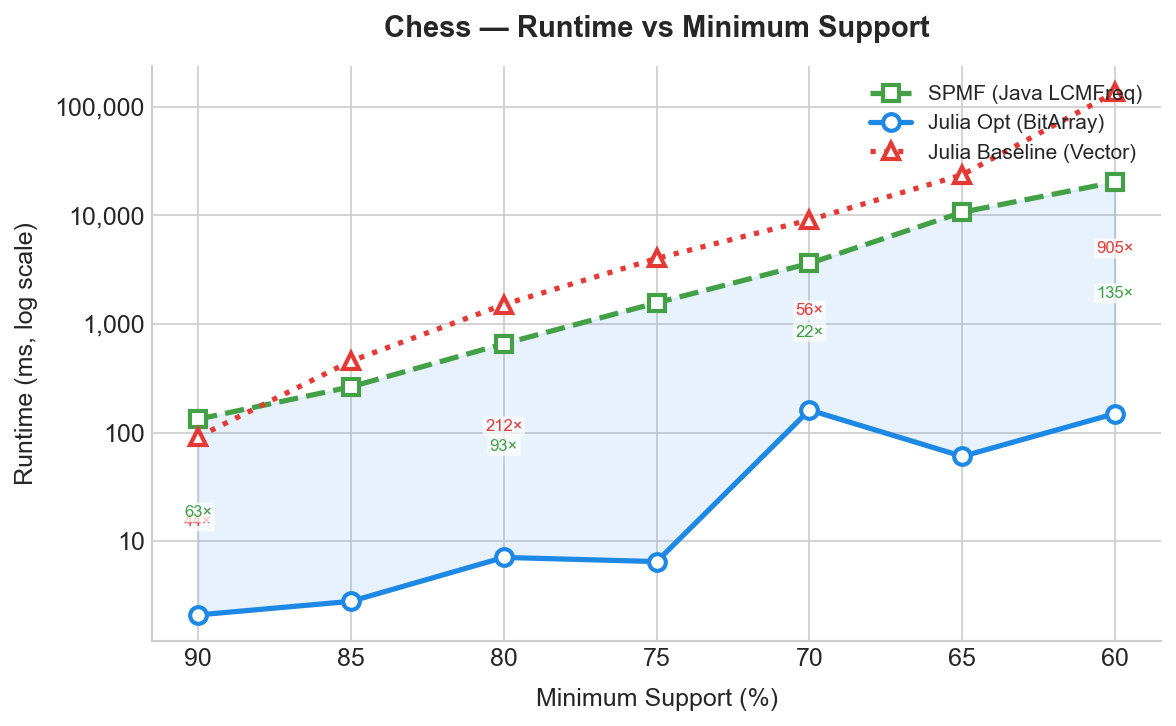
\includegraphics[width=\linewidth]{../data/results/figures/runtime_chess.png}\\
    \small Chess (dày đặc)
    \column{0.48\textwidth}
    \centering
    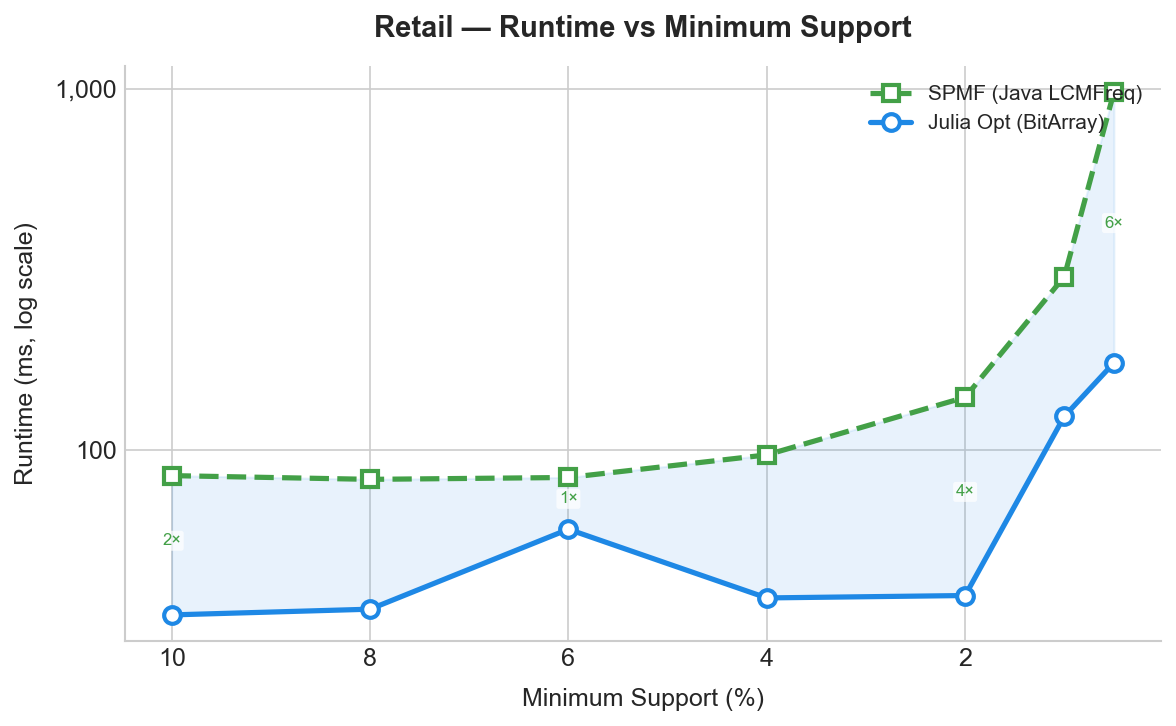
\includegraphics[width=\linewidth]{../data/results/figures/runtime_retail.png}\\
    \small Retail (thưa)
  \end{columns}
  \vspace{0.2em}
  \small Chess: nhanh hơn SPMF $76$--$141\times$. Retail: $2$--$6\times$
  (denotation đã nhỏ sẵn). Baseline OOM trên Retail (16\,470 item).
\end{frame}

\begin{frame}{Tăng tốc so với SPMF}
  \begin{columns}[T,onlytextwidth]
    \column{0.46\textwidth}
    \small
    \begin{tabular}{@{}lrrr@{}}
      \toprule Dataset & Trung vị & Min & Max \\ \midrule
      Chess       & $135\times$ & $22\times$ & $241\times$ \\
      Pumsb       & $343\times$ & $12\times$ & $343\times$ \\
      Mushroom    & $58\times$  & $23\times$ & $101\times$ \\
      T40I10D100K & $32\times$  & $21\times$ & $32\times$ \\
      Connect     & $6\times$   & $1\times$  & $34\times$ \\
      Retail      & $2\times$   & $1\times$  & $6\times$ \\
      \bottomrule
    \end{tabular}
    \column{0.50\textwidth}
    \centering
    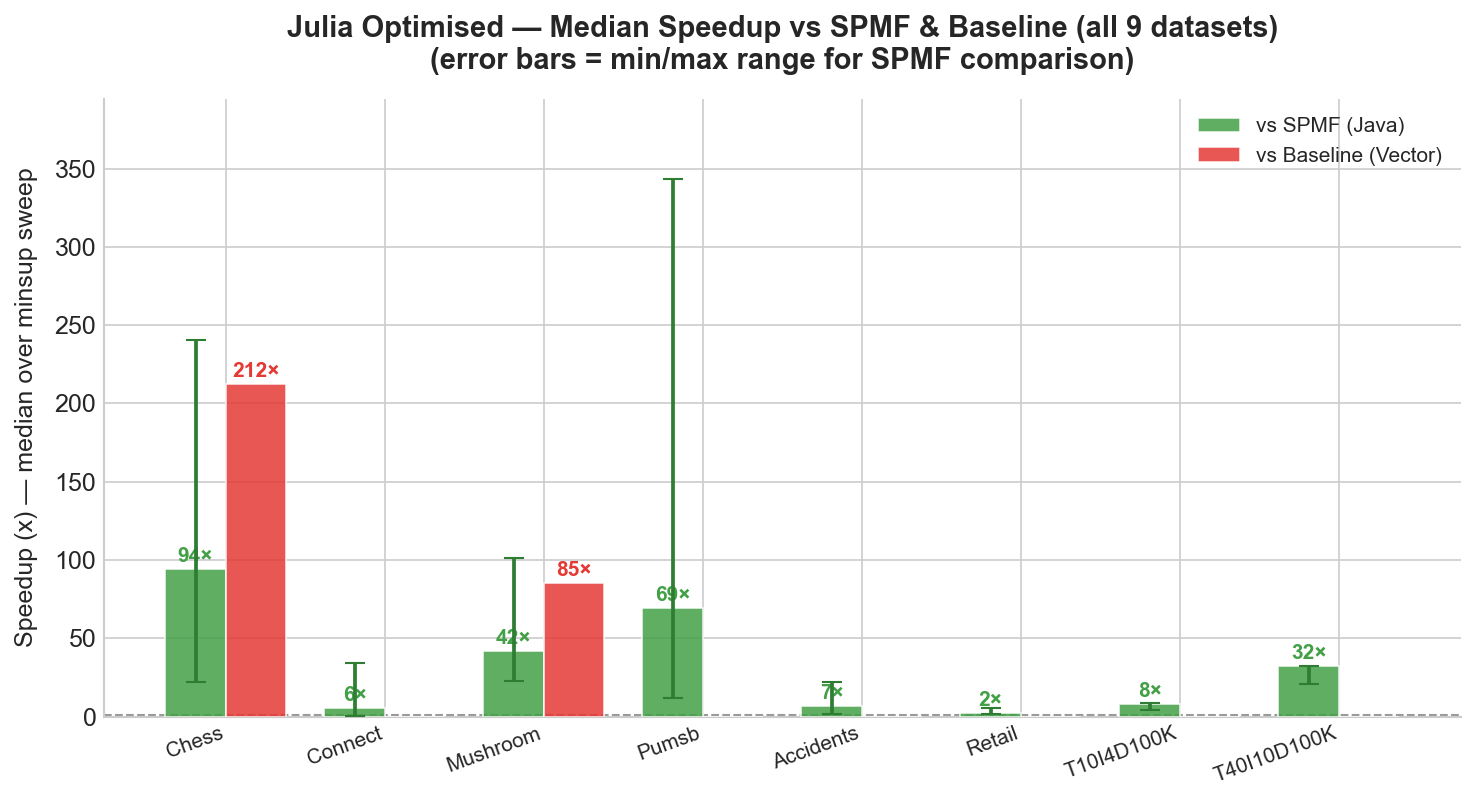
\includegraphics[width=\linewidth]{../data/results/figures/speedup_bar.png}
  \end{columns}
  \vspace{0.1em}
  \small Pumsb cao nhất nhờ giao dịch dài (74 item) $\Rightarrow$ AND bit
  khuếch đại lợi thế.
\end{frame}

\begin{frame}{Số lượng frequent itemset \& bộ nhớ}
  \begin{columns}[T,onlytextwidth]
    \column{0.48\textwidth}
    \centering
    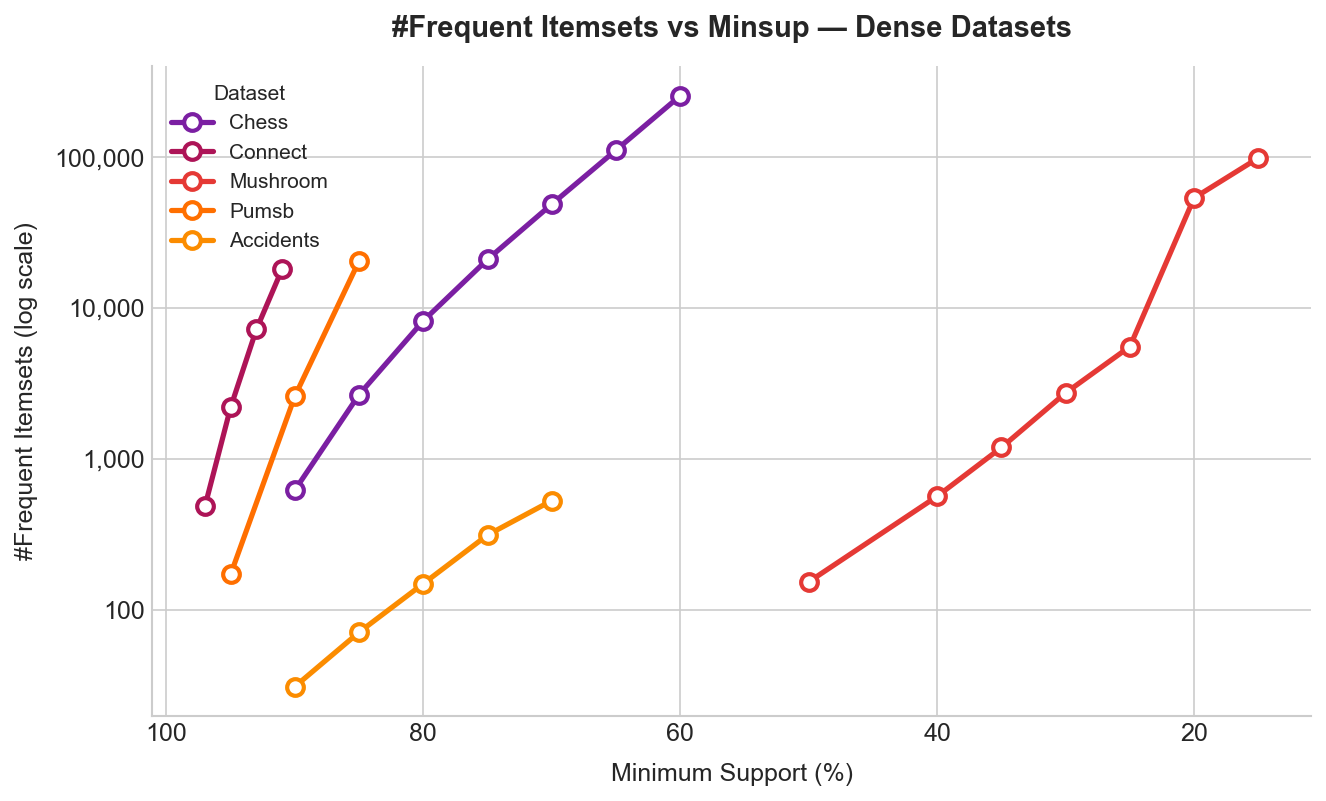
\includegraphics[width=\linewidth]{../data/results/figures/itemsets_dense.png}\\
    \small Số itemset theo minsup (dataset dày đặc)
    \column{0.48\textwidth}
    \small
    \begin{tabular}{@{}lrrr@{}}
      \toprule Dataset & Opt (MiB) & Baseline & Giảm \\ \midrule
      Chess       & 31.87  & 857.23 & $26.9\times$ \\
      Mushroom    & 10.98  & 161.57 & $14.7\times$ \\
      Retail      & 20.68  & OOM    & N/A \\
      T10I4D100K  & 1\,215.2 & OOM  & N/A \\
      \bottomrule
    \end{tabular}
    \vspace{0.3em}\\
    \footnotesize BitArray: 1 bit/transaction (vs.\ 8 byte/TID ở
    \texttt{Vector\{Int\}}) $\Rightarrow$ tiết kiệm $\sim 64\times$ mỗi
    denotation.
  \end{columns}
\end{frame}

\begin{frame}{Khả năng mở rộng \& ảnh hưởng độ dài giao dịch}
  \begin{columns}[T,onlytextwidth]
    \column{0.48\textwidth}
    \centering
    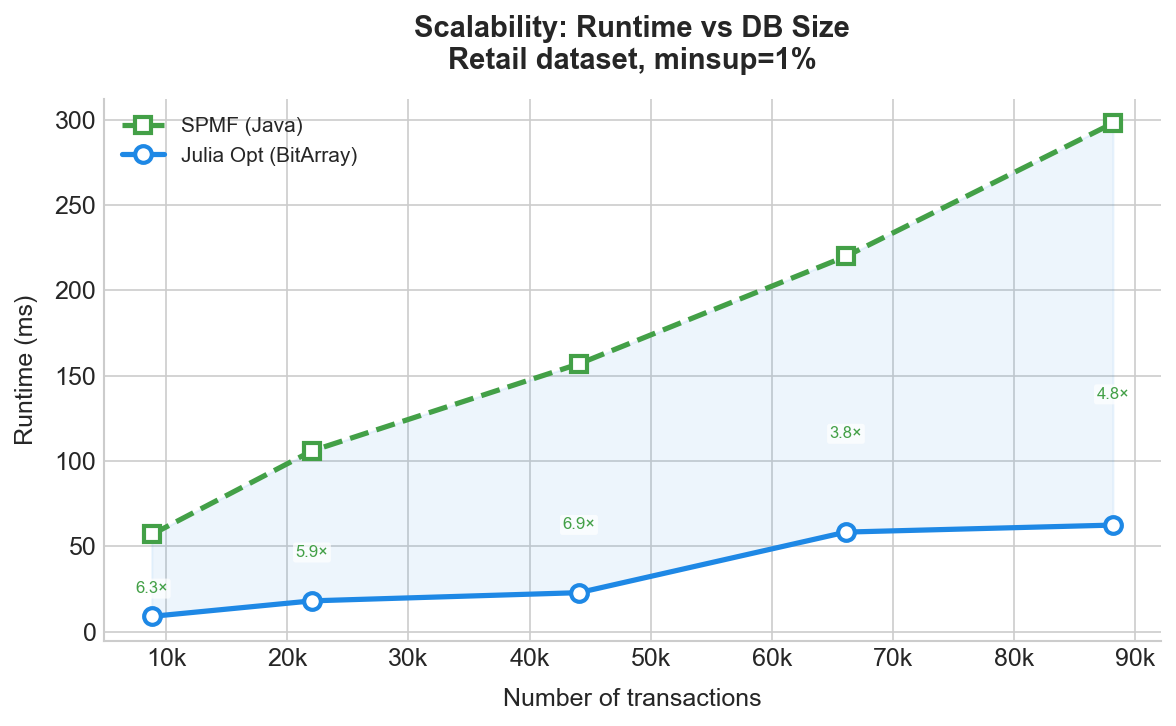
\includegraphics[width=\linewidth]{../data/results/figures/scalability_by_ntx.png}\\
    \small Retail, lấy mẫu theo tỉ lệ — thời gian chạy gần tuyến tính theo
    số giao dịch.
    \column{0.48\textwidth}
    \centering
    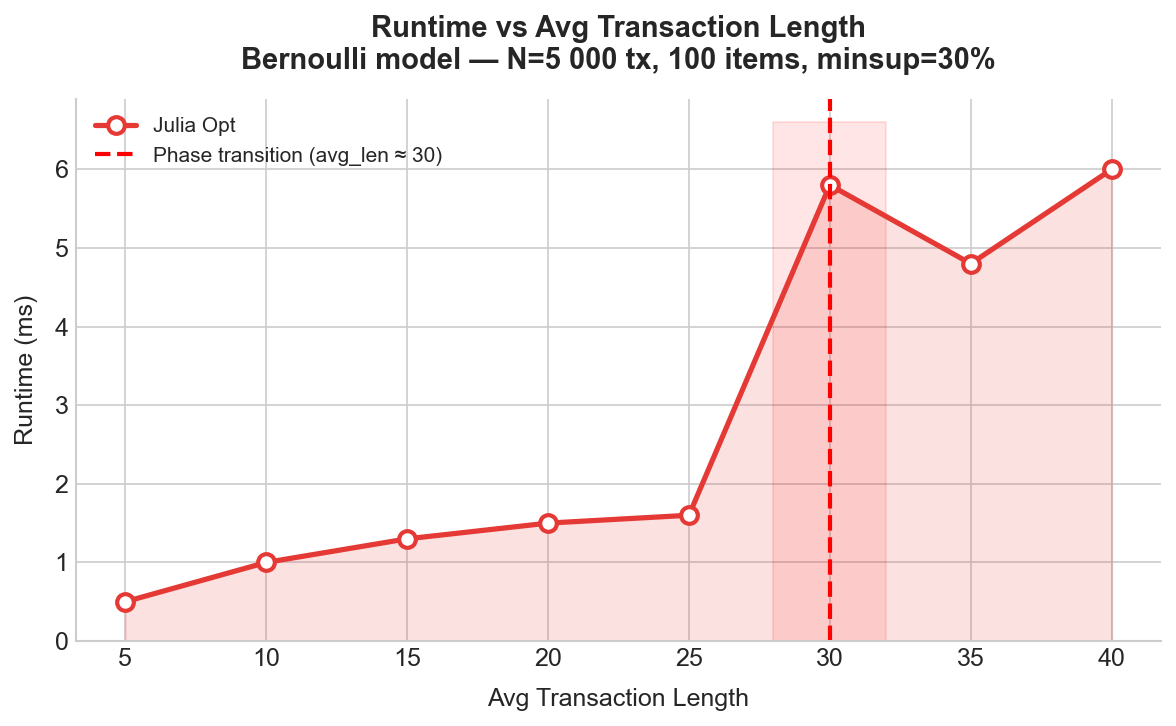
\includegraphics[width=\linewidth]{../data/results/figures/txlen_runtime.png}\\
    \small Dataset tổng hợp: khi độ dài TB vượt ngưỡng pha chuyển
    ($\approx 30$), itemset phổ biến xuất hiện đột ngột.
  \end{columns}
\end{frame}

% ===================================================================
\section{Ứng dụng: phân tích giỏ hàng}
% ===================================================================

\begin{frame}{Sinh luật kết hợp từ kết quả LCMFreq}
  Với itemset $X$ frequent, $Y\subset X$:
  \begin{equation}
    \mathrm{conf}(Y\Rightarrow X\setminus Y)=\frac{\mathrm{sup}(X)}{\mathrm{sup}(Y)}\geq\text{minconf},
    \qquad \mathrm{lift}>1 \Rightarrow \text{đồng xuất hiện nhiều hơn ngẫu nhiên}.
  \end{equation}
  \small Retail (88\,162 giao dịch): minsup$=0.5\%$ ($\sigma=441$) $\to$ 580
  frequent itemset; minconf$=60\%$ $\to$ 312 association rule.

  \vspace{0.4em}
  \centering\small
  \begin{tabular}{@{}llrrr@{}}
    \toprule Vế trái & Vế phải & Support & Conf. & Lift \\ \midrule
    $\{38,39\}$ & $\{41\}$    & 1.01\% & 0.89 & 8.7 \\
    $\{38\}$    & $\{39,41\}$ & 1.01\% & 0.82 & 8.1 \\
    $\{39\}$    & $\{38\}$    & 1.18\% & 0.73 & 7.2 \\
    $\{32\}$    & $\{48\}$    & 0.72\% & 0.78 & 6.4 \\
    \bottomrule
  \end{tabular}\\
  \vspace{0.2em}
  \footnotesize\color{black!55} Nhóm $\{38,39,41\}$: lift $>7$ — ứng viên
  mạnh cho bán theo gói / bố trí gần nhau.
\end{frame}

% ===================================================================
\section{Kết luận}
% ===================================================================

\begin{frame}{Kết luận}
  \begin{columns}[T]
    \column{0.34\textwidth}
    \small\textbf{Đã hoàn thành}
    \begin{itemize}
      \item Backtracking + OccurrenceDeliver + Hypercube theo Uno et al.\ (2004)
      \item \opt{Bản tối ưu BitArray}, unit test tự động
      \item Khớp 100\% với SPMF (9 dataset)
      \item Ứng dụng giỏ hàng trên Retail
    \end{itemize}
    \column{0.32\textwidth}
    \small\textbf{Giới hạn}
    \begin{itemize}
      \item Bộ nhớ còn cao trên T10I4D100K ($\sim$1.2 GiB)
      \item Chưa dùng diffset
      \item Chưa song song hóa DFS
    \end{itemize}
    \column{0.32\textwidth}
    \small\textbf{Hướng phát triển}
    \begin{itemize}
      \item Diffset để giảm bộ nhớ
      \item Đa luồng cho nhánh top-level
      \item Mở rộng sang closed/maximal itemset
    \end{itemize}
  \end{columns}
  \vspace{0.4em}
  \begin{alertblock}{Tóm lại}
    Backtracking tiết kiệm bộ nhớ so với Apriori; OccurrenceDeliver khắc
    phục điểm yếu đếm support của backtracking; Hypercube giảm số lần đếm
    lặp lại. Bản tối ưu BitArray giữ nguyên khung sinh itemset, chỉ đổi
    cấu trúc denotation — \opt{đóng góp riêng của nhóm}, không sao chép từ
    SPMF (SPMF chỉ dùng để đối chiếu kết quả).
  \end{alertblock}
\end{frame}

\begin{frame}{Tài liệu tham khảo}
  \footnotesize
  \begin{enumerate}
    \item T. Uno, M. Kiyomi, H. Arimura. \textit{LCM ver.2: Efficient Mining
      Algorithms for Frequent/Closed/Maximal Itemsets}. IEEE ICDM Workshop on
      FIMI, Brighton, UK, 2004.
    \item R. Agrawal, R. Srikant. \textit{Fast Algorithms for Mining
      Association Rules}. Proc. 20th VLDB, pp. 487--499, 1994.
    \item J. Han, J. Pei, Y. Yin. \textit{Mining Frequent Patterns without
      Candidate Generation}. Proc. ACM SIGMOD, pp. 1--12, 2000.
    \item M. J. Zaki et al. \textit{New Algorithms for Fast Discovery of
      Association Rules}. Proc. 3rd KDD, pp. 283--286, 1997.
  \end{enumerate}
\end{frame}

\begin{frame}[standout]
  \centering
  \Large Cảm ơn thầy/cô và các bạn!\\[0.8em]
  \normalsize Câu hỏi?\\[1.5em]
  \footnotesize Nhóm 01, CSC14004 \quad|\quad
  Trường Đại học Khoa học Tự nhiên, ĐHQG-HCM
\end{frame}

\end{document}
